
%(BEGIN_QUESTION)
% Copyright 2015, Tony R. Kuphaldt, released under the Creative Commons Attribution License (v 1.0)
% This means you may do almost anything with this work of mine, so long as you give me proper credit

Examine this ``live'' display of a FOUNDATION Fieldbus control strategy where multiple temperature transmitters are used to redundantly measure the same physical point in a chemical reactor:

$$\includegraphics[width=15.5cm]{i02550x01.eps}$$

Based on the signal values shown in this ``live'' display of the function block diagram, identify the selection type parameter value ({\tt SEL\_TYPE}) set in the ISEL function block.

\vskip 10pt

Also, explain how such a ``live'' display of a control system's function block diagram could be useful as a diagnostic tool, if you were tasked with troubleshooting a malfunctioning process control loop.

\vskip 20pt \vbox{\hrule \hbox{\strut \vrule{} {\bf Suggestions for Socratic discussion} \vrule} \hrule}

\begin{itemize}
\item{} Identify the value output by the ISEL block if its {\tt SEL\_TYPE} parameter were set differently.
\item{} How would a faulted temperature sensor be revealed in this ``live'' function block diagram display?
\item{} How would a faulted final control element be revealed in this ``live'' function block diagram display?
\item{} How would a PID function block left in manual mode be revealed in this ``live'' function block diagram display?
\item{} Identify the effect(s) of placing the lower AI function block in ``OOS'' mode.
\item{} Identify the effect(s) of placing the ISEL function block in ``OOS'' mode.
\item{} Identify the effect(s) of placing the AO function block in ``OOS'' mode.
\item{} Identify the effect(s) of placing the upper AI function block in ``manual'' mode.
\item{} Identify the effect(s) of placing the ISEL function block in ``manual'' mode.
\item{} Identify the effect(s) of placing the AO function block in ``manual'' mode.
\end{itemize}

\underbar{file i02550}
%(END_QUESTION)





%(BEGIN_ANSWER)

I won't reveal any answers here, but I will suggest you explore the ``Online'' mode in the Emerson DeltaV DCS Control Studio utility to see a working example of how live signal values may be displayed in a function block diagram.

%(END_ANSWER)





%(BEGIN_NOTES)

The {\tt SEL\_TYPE} parameter is set to {\it avg} (average) in this function block program, as revealed by the value of the ISEL block's output compared to its three input values.  Available selection types provided by the ISEL function block include:

\begin{itemize}
\item{} {\bf max} (maximum input value)
\item{} {\bf min} (minimum input value)
\item{} {\bf avg} (average of all input values)
\item{} {\bf mid} (middle of three input values, or average of middle two input values)
\item{} {\bf 1st good} (first input value with a ``good'' status)
\item{} {\bf hot backup} (stays with selected input until that input registers a ``bad'' status)
\end{itemize}


%INDEX% Control, strategies: selector (using ISEL Fieldbus function block)
%INDEX% DCS, programming: function block program

%(END_NOTES)


